% Mid-Semester Project Report — EESD for Hindi
% ACL 2023 Style Template
\documentclass[11pt]{article}
% For Hindi Unicode support, use XeLaTeX or LuaLaTeX and these packages:
\usepackage{fontspec}
\usepackage{polyglossia}
\setmainlanguage{english}
\setotherlanguage{hindi}
\newfontfamily\devanagarifont[Script=Devanagari]{Noto Sans Devanagari}
% Set main font for English (supports bold/italic)
\setmainfont{Latin Modern Roman}
% Optionally, set sans-serif and monospaced fonts if needed:
% \setsansfont{Latin Modern Sans}
% \setmonofont{Latin Modern Mono}
\usepackage[hyperref]{acl}
\usepackage{latexsym}
\usepackage{graphicx}
\usepackage{amsmath}
\usepackage{amssymb}
\usepackage{booktabs}
\usepackage{multirow}
\usepackage{subcaption}
\usepackage{url}
\usepackage{xcolor}
%\usepackage{algorithm}
%\usepackage{algpseudocode}

\aclfinalcopy

\title{Early-Exit Speculative Decoding for Hindi: \\
An Empirical Study on Morphologically Rich Languages}

\author{
\textbf{Team: Transformers} \\
KSPSVLN Siddardha Kumar Kavuri (2025201061) \\
Piyush Kumar Agarwal (2025201082) \\
Sankalp Chaturvedi (2025201083) \\
Aviral Tyagi (2025201086)
}


\date{}

\begin{document}
\maketitle

% ===================================================================
\begin{abstract}
Autoregressive decoding in large language models (LLMs) is inherently sequential and slow, with each token requiring a full forward pass through all transformer layers.  Speculative decoding alleviates this by using a lightweight \emph{draft} model to propose multiple tokens that the full model then verifies in a single pass.  However, maintaining a separate draft model doubles parameter storage and complicates deployment.

We implement \textbf{Early-Exit Speculative Decoding (EESD)}, which eliminates the need for a separate draft model by attaching lightweight exit heads at intermediate transformer layers of the target model itself.  We apply EESD to \textbf{Qwen2-1.5B} for \textbf{Hindi text generation}, training exit heads at layers 8, 16, and 22 of the 28-layer architecture using KL-divergence distillation on \textbf{167K Hindi sentences} from AI4Bharat IndicCorpv2.

After 10 epochs of training, our system achieves a mean acceptance rate of $\alpha = 0.646$ at depth 22 on 101 Hindi prompts, with a wall-clock speedup of $0.47\times$ relative to standard autoregressive decoding.  While the current speedup is below $1\times$ due to the lack of true early-exit inference (the full model still runs all layers during drafting), the high acceptance rates demonstrate that the exit heads successfully approximate the full model's distribution, validating the approach for future deployment with optimised inference kernels.
\end{abstract}

% ===================================================================
\section{Introduction}
\label{sec:intro}

Large Language Models (LLMs) underpin modern NLP applications from machine translation to dialogue systems \cite{zhou2024survey}.  Despite their effectiveness, inference remains compute-bound: generating $N$ tokens requires $N$ sequential forward passes, each traversing every transformer layer.  For a 28-layer model producing 100 tokens, this amounts to 2,800 layer evaluations with no parallelism across the token dimension.

\textbf{Speculative decoding} \cite{leviathan2023fast,chen2023accelerating} addresses this bottleneck by introducing a two-phase generate-then-verify paradigm.  A small, fast \emph{draft model} proposes $K$ candidate tokens, which the larger \emph{target model} verifies in a single batched forward pass.  Accepted tokens bypass the sequential bottleneck, yielding wall-clock speedups of $2$--$3\times$ without changing the output distribution.

A key limitation of vanilla speculative decoding is the requirement for a separate draft model that must (i) be small enough to be fast, (ii) produce a token distribution close to the target, and (iii) be stored alongside the target model, roughly doubling memory requirements.

\textbf{Early-Exit Speculative Decoding} (EESD) \cite{liu2024eesd} resolves all three issues by reusing the target model's own intermediate representations.  Lightweight ``exit heads''—comprising a LayerNorm and a linear projection—are attached at selected intermediate layers.  During drafting, inference can in principle stop at the exit layer rather than running all layers, providing both speed and distribution alignment with zero additional model parameters beyond the small heads.

In this project, we implement EESD for \textbf{Hindi text generation} using \textbf{Qwen2-1.5B} \cite{yang2024qwen2} as the base model.  Hindi serves as an interesting testbed because its rich morphology (inflected verbs, compound words, postpositions) presents a real challenge for draft-model accuracy.

\paragraph{Contributions.}
\begin{enumerate}
    \item A complete, open-source EESD implementation for Qwen2-1.5B with exit heads at layers 8, 16, and 22.
    \item Training via KL-divergence soft distillation \cite{hinton2015distilling} on 167K Hindi sentences from AI4Bharat IndicCorpv2 \cite{doddapaneni2021indicnlp}.
    \item Comprehensive evaluation on 101 Hindi prompts across three draft depths, analysing acceptance rate, speedup, and token-level statistics.
    \item Analysis of the depth--accuracy trade-off and discussion of the gap between simulated and true early-exit inference.
\end{enumerate}


% ===================================================================
\section{Background and Related Work}
\label{sec:background}

\subsection{Autoregressive Decoding}

Standard autoregressive (AR) generation produces one token at a time: $x_t \sim p_\theta(x_t \mid x_{<t})$.  Each step requires a full forward pass through all $L$ transformer layers.  For a model with $L = 28$ layers generating $N = 100$ tokens, this means $28 \times 100 = 2{,}800$ sequential layer evaluations—a major bottleneck, especially on resource-constrained hardware.

\subsection{Speculative Decoding}

Speculative decoding \cite{leviathan2023fast,chen2023accelerating,stern2018blockwise} introduces a \emph{draft-then-verify} paradigm:
\begin{enumerate}
    \item A lightweight draft model $q_\phi$ generates $K$ candidate tokens autoregressively.
    \item The full target model $p_\theta$ processes the prompt plus all $K$ candidates in a single forward pass.
    \item Tokens are accepted greedily until the first mismatch; the correct token at the mismatch position is sampled from $p_\theta$.
\end{enumerate}

If the draft model's acceptance rate is $\alpha$, the expected number of accepted tokens per verification step is $\frac{\alpha(1 - \alpha^K)}{1 - \alpha}$, yielding a speedup proportional to $K \cdot \alpha$ when draft generation is much cheaper than target verification \cite{xia2024unlocking}.

Variants include Big Little Decoder \cite{kim2024speculative}, which uses a smaller model from the same family, Medusa \cite{cai2023medusa}, which adds multiple prediction heads for future positions, and Draft \& Verify \cite{zhang2023draft}, which achieves lossless acceleration via self-speculative decoding.  Yan et al.~\cite{yan2025decoding} provide a thorough analysis of speculative decoding, while Zhao et al.~\cite{zhao2025frspec} improve efficiency through frequency-ranked speculative sampling.

\subsection{Early Exiting for Language Models}

Early exiting attaches classifiers at intermediate layers and routes easy inputs to shallow exits.  BranchyNet \cite{teerapittayanon2016branchynet} pioneered this for CNNs; DeeBERT \cite{xin2020deebert} and CALM \cite{schuster2022confident} adapted the idea for BERT and decoder-only transformers respectively.  Bae et al.~\cite{bae2023fast} propose a synchronized parallel decoding framework for fast and robust early exiting in autoregressive models.

\subsection{EESD: Early-Exit Speculative Decoding}

Liu et al.~\cite{liu2024eesd} combine early exiting with speculative decoding.  Instead of maintaining a separate draft model, they attach exit heads at intermediate layers of the target LLM.  The shallowest exit head serves as the draft model, generating $K$ tokens using only the first $d$ layers.  The full model then verifies all $K$ tokens in one pass.

Key advantages:
\begin{itemize}
    \item \textbf{No external draft model}: exit heads add $< 0.5\%$ parameters.
    \item \textbf{Inherent distribution alignment}: intermediate representations already encode significant information about the target distribution.
    \item \textbf{Flexible depth selection}: multiple exit heads at different depths allow trading off draft speed versus acceptance rate.
\end{itemize}

The original paper further introduces a Thompson Sampling mechanism to dynamically select the optimal exit depth at each decoding step, maximising the expected speedup.  In this project, we focus on the core EESD mechanism with fixed exit depths.  Related concurrent approaches include LayerSkip \cite{elhoushi2024layerskip}, which combines layer dropout during training with self-speculative decoding, Kangaroo \cite{liu2024kangaroo}, which achieves lossless self-speculative decoding via double early exiting, and SpecEE \cite{xu2025specee}, which introduces speculative early exiting at the hardware architecture level.


% ===================================================================
\section{Dataset}
\label{sec:dataset}

\subsection{Training Data: AI4Bharat IndicCorpv2}

We use the Hindi subset of \textbf{AI4Bharat IndicCorpv2} \cite{doddapaneni2021indicnlp}, a large-scale monolingual corpus for Indian languages.  The Hindi portion comprises three text files (\texttt{hi-1.txt}, \texttt{hi-2.txt}, \texttt{hi-3.txt}) totalling approximately 27~GB each.  We sample \textbf{167,000 sentences} ($\approx$5M tokens at an average of 30 tokens per sentence), following the scale used in the original EESD paper.

All sentences are tokenised using the Qwen2 tokenizer (BPE-based, vocabulary size 151,936) with a maximum sequence length of 256 tokens, padded and truncated as needed.

\subsection{Evaluation Data}

For large-scale inference evaluation, we curate \textbf{101 diverse Hindi prompts} spanning topics including Indian geography, culture, history, science, politics, sports, economy, and daily life.  These prompts range from 10 to 25 tokens and are designed to elicit varied morphological structures.

For the formal depth analysis and morphological evaluation, we additionally use the test split of \textbf{XL-Sum Hindi} \cite{hasan2021xlsum}, a BBC multilingual summarisation dataset, which provides clean, naturally-occurring Hindi text.


% ===================================================================
\section{Methodology}
\label{sec:methodology}

\subsection{Architecture}

\paragraph{Base Model.}  We use \textbf{Qwen2-1.5B} \cite{yang2024qwen2}, a 28-layer transformer decoder with hidden dimension 1,536 and vocabulary size 151,936.  The model is loaded in float16 precision with \texttt{device\_map="auto"} and all base parameters are \emph{frozen} throughout training.

\paragraph{Exit Heads.}  At each selected layer depth $d \in \{8, 16, 22\}$, we attach a lightweight exit head consisting of:
\begin{equation}
    \hat{y}_d = \text{Linear}\bigl(\text{LayerNorm}(h_d)\bigr)
\end{equation}
where $h_d \in \mathbb{R}^{B \times T \times 1536}$ is the hidden state after the $d$-th transformer layer, and the linear projection maps to the full vocabulary size.  Each exit head adds approximately \textbf{233M parameters} ($1536 \times 151936 + 1536$), but since these are the only trainable parameters, the training memory footprint is minimal.

\paragraph{Exit Depth Selection.}  The three depths—8, 16, 22—are chosen to span the model:
\begin{itemize}
    \item \textbf{Layer 8} (shallow, $\sim\frac{1}{3}$ depth): fastest draft but lowest accuracy.
    \item \textbf{Layer 16} (mid, $\sim\frac{1}{2}$ depth): moderate speed--accuracy trade-off.
    \item \textbf{Layer 22} (deep, $\sim\frac{3}{4}$ depth): closest to full model, highest acceptance rate.
\end{itemize}

\subsection{Training Objective}

We train the exit heads using \textbf{soft KL-divergence distillation} \cite{hinton2015distilling}.  The frozen full model serves as the teacher:
\begin{equation}
    \mathcal{L} = \frac{1}{|\mathcal{D}|} \sum_{d \in \mathcal{D}} T^2 \cdot D_{\text{KL}}\bigl(\sigma(f / T) \;\|\; \sigma(\hat{f}_d / T)\bigr)
\label{eq:loss}
\end{equation}
where $\mathcal{D} = \{8, 16, 22\}$ is the set of exit depths, $f$ and $\hat{f}_d$ are the full-model and exit-head logits respectively, $T = 2.0$ is the distillation temperature, and $\sigma$ denotes softmax.

The $T^2$ scaling factor \cite{hinton2015distilling} compensates for the reduced gradient magnitude at higher temperatures, keeping the effective learning rate consistent.  Soft targets transfer the full probability distribution—not just the argmax—providing richer supervision than hard label matching.

\subsection{Training Setup}

\begin{itemize}
    \item \textbf{Optimiser:} 8-bit AdamW \cite{loshchilov2019adamw} via \texttt{bitsandbytes}, saving $\sim$4~GB VRAM.
    \item \textbf{Learning rate:} $10^{-4}$ with cosine annealing and 5\% linear warmup.
    \item \textbf{Batch size:} 2 per GPU with gradient accumulation of 4 (effective batch size 8).
    \item \textbf{Epochs:} 10 (167K samples per epoch, $\sim$41{,}750 steps per epoch).
    \item \textbf{Hardware:} NVIDIA T4 16~GB (Kaggle) for primary training; Colab A100 for inference.
    \item \textbf{Precision:} float16 base model, float32 loss computation for numerical stability.  BF16 autocast on Ampere+ GPUs.
\end{itemize}

Implementation uses forward hooks to capture intermediate hidden states during a single base-model forward pass, avoiding manual layer-by-layer iteration that would break attention mask preparation and rotary positional embeddings.

% ---------------------------------------------------------------
\subsection{Performance Metrics}
\label{sec:performance_metrics}

We report the following key performance metrics to evaluate the effectiveness of Early-Exit Speculative Decoding (EESD):
\begin{itemize}
\item \textbf{Acceptance Rate (
α
α):} The proportion of draft tokens generated by the exit head that are accepted by the full model during verification. Higher 
α
α indicates better alignment between the exit head and the full model.
\item \textbf{Speedup:} The ratio of wall-clock time for EESD decoding to standard autoregressive decoding. Speedup 
>
1
>1 indicates faster inference.
\item \textbf{EESD Inference Time:} Average time (in seconds) taken to generate outputs using EESD for a fixed number of tokens and prompts.
\item \textbf{Autoregressive (AR) Inference Time:} Average time (in seconds) for standard AR decoding under the same conditions.
\item \textbf{Tokens Accepted/Drafted:} The total number of tokens accepted and drafted during EESD inference, providing insight into efficiency and draft quality.
\item \textbf{Depth-wise Metrics:} All metrics are reported for each exit head depth (8, 16, 22) to analyse the trade-off between speed and accuracy.
\end{itemize}

These metrics are summarised in Tables\ref{tab:inference_main} and \ref{tab:formal_eval}, and visualised in Figures\ref{fig:loss_plots} and \ref{fig:inference_comparison}.
% ---------------------------------------------------------------


\subsection{Inference: Speculative Decoding Loop}

At inference time, EESD follows the standard speculative decoding protocol:

\noindent\fbox{\parbox{0.96\columnwidth}{
\textbf{Algorithm: EESD Speculative Decoding} \\[4pt]
\textbf{Input:} Model $M$ with exit head at depth $d$, prompt $x_{1:n}$, draft length $K$, max\_new\_tokens $N$ \\[4pt]
\begin{tabular}{@{}r@{\;}p{0.85\columnwidth}@{}}
1. & $\text{generated} \leftarrow x_{1:n}$ \\[2pt]
2. & \textbf{While} $|\text{generated}| - n < N$: \\[2pt]
3. & \hspace{1em}\textbf{Draft:} For $k = 1 \ldots K$: \\[2pt]
4. & \hspace{2em}Run forward pass, hook hidden state at layer $d$ \\[2pt]
5. & \hspace{2em}$\hat{x}_{n+k} \leftarrow \arg\max\;\text{ExitHead}_d(h_d^{(n+k-1)})$ \\[2pt]
6. & \hspace{1em}\textbf{Verify:} Run full model on $[\text{generated}; \hat{x}_{n+1:n+K}]$ \\[2pt]
7. & \hspace{1em}Accept tokens until first mismatch \\[2pt]
8. & \hspace{1em}Append accepted tokens to generated \\
\end{tabular}
}}

\paragraph{Important caveat.}  In our current implementation, drafting still runs the full base model (all 28 layers) during each draft step, with a forward hook capturing the hidden state at the exit layer.  The exit head produces the draft token from this intermediate representation, but the computational cost of the full forward pass is still incurred.  A production deployment would require custom CUDA kernels or model surgery to truly exit early.  Our results therefore measure the \emph{quality} of exit-head predictions (acceptance rate) rather than the true latency speedup achievable with optimised early-exit inference.


% ===================================================================
\section{Experiments and Results}
\label{sec:results}

\subsection{Training Convergence}

We trained for 10 epochs on 167K Hindi sentences.  Figure~\ref{fig:loss_plots} presents all training curves: (a)~overall loss, (b)~per-depth training loss, (c)~per-depth validation loss, and (d)~acceptance rate on a subset of validation set prompts during training.

\begin{figure*}[p]
    \centering
    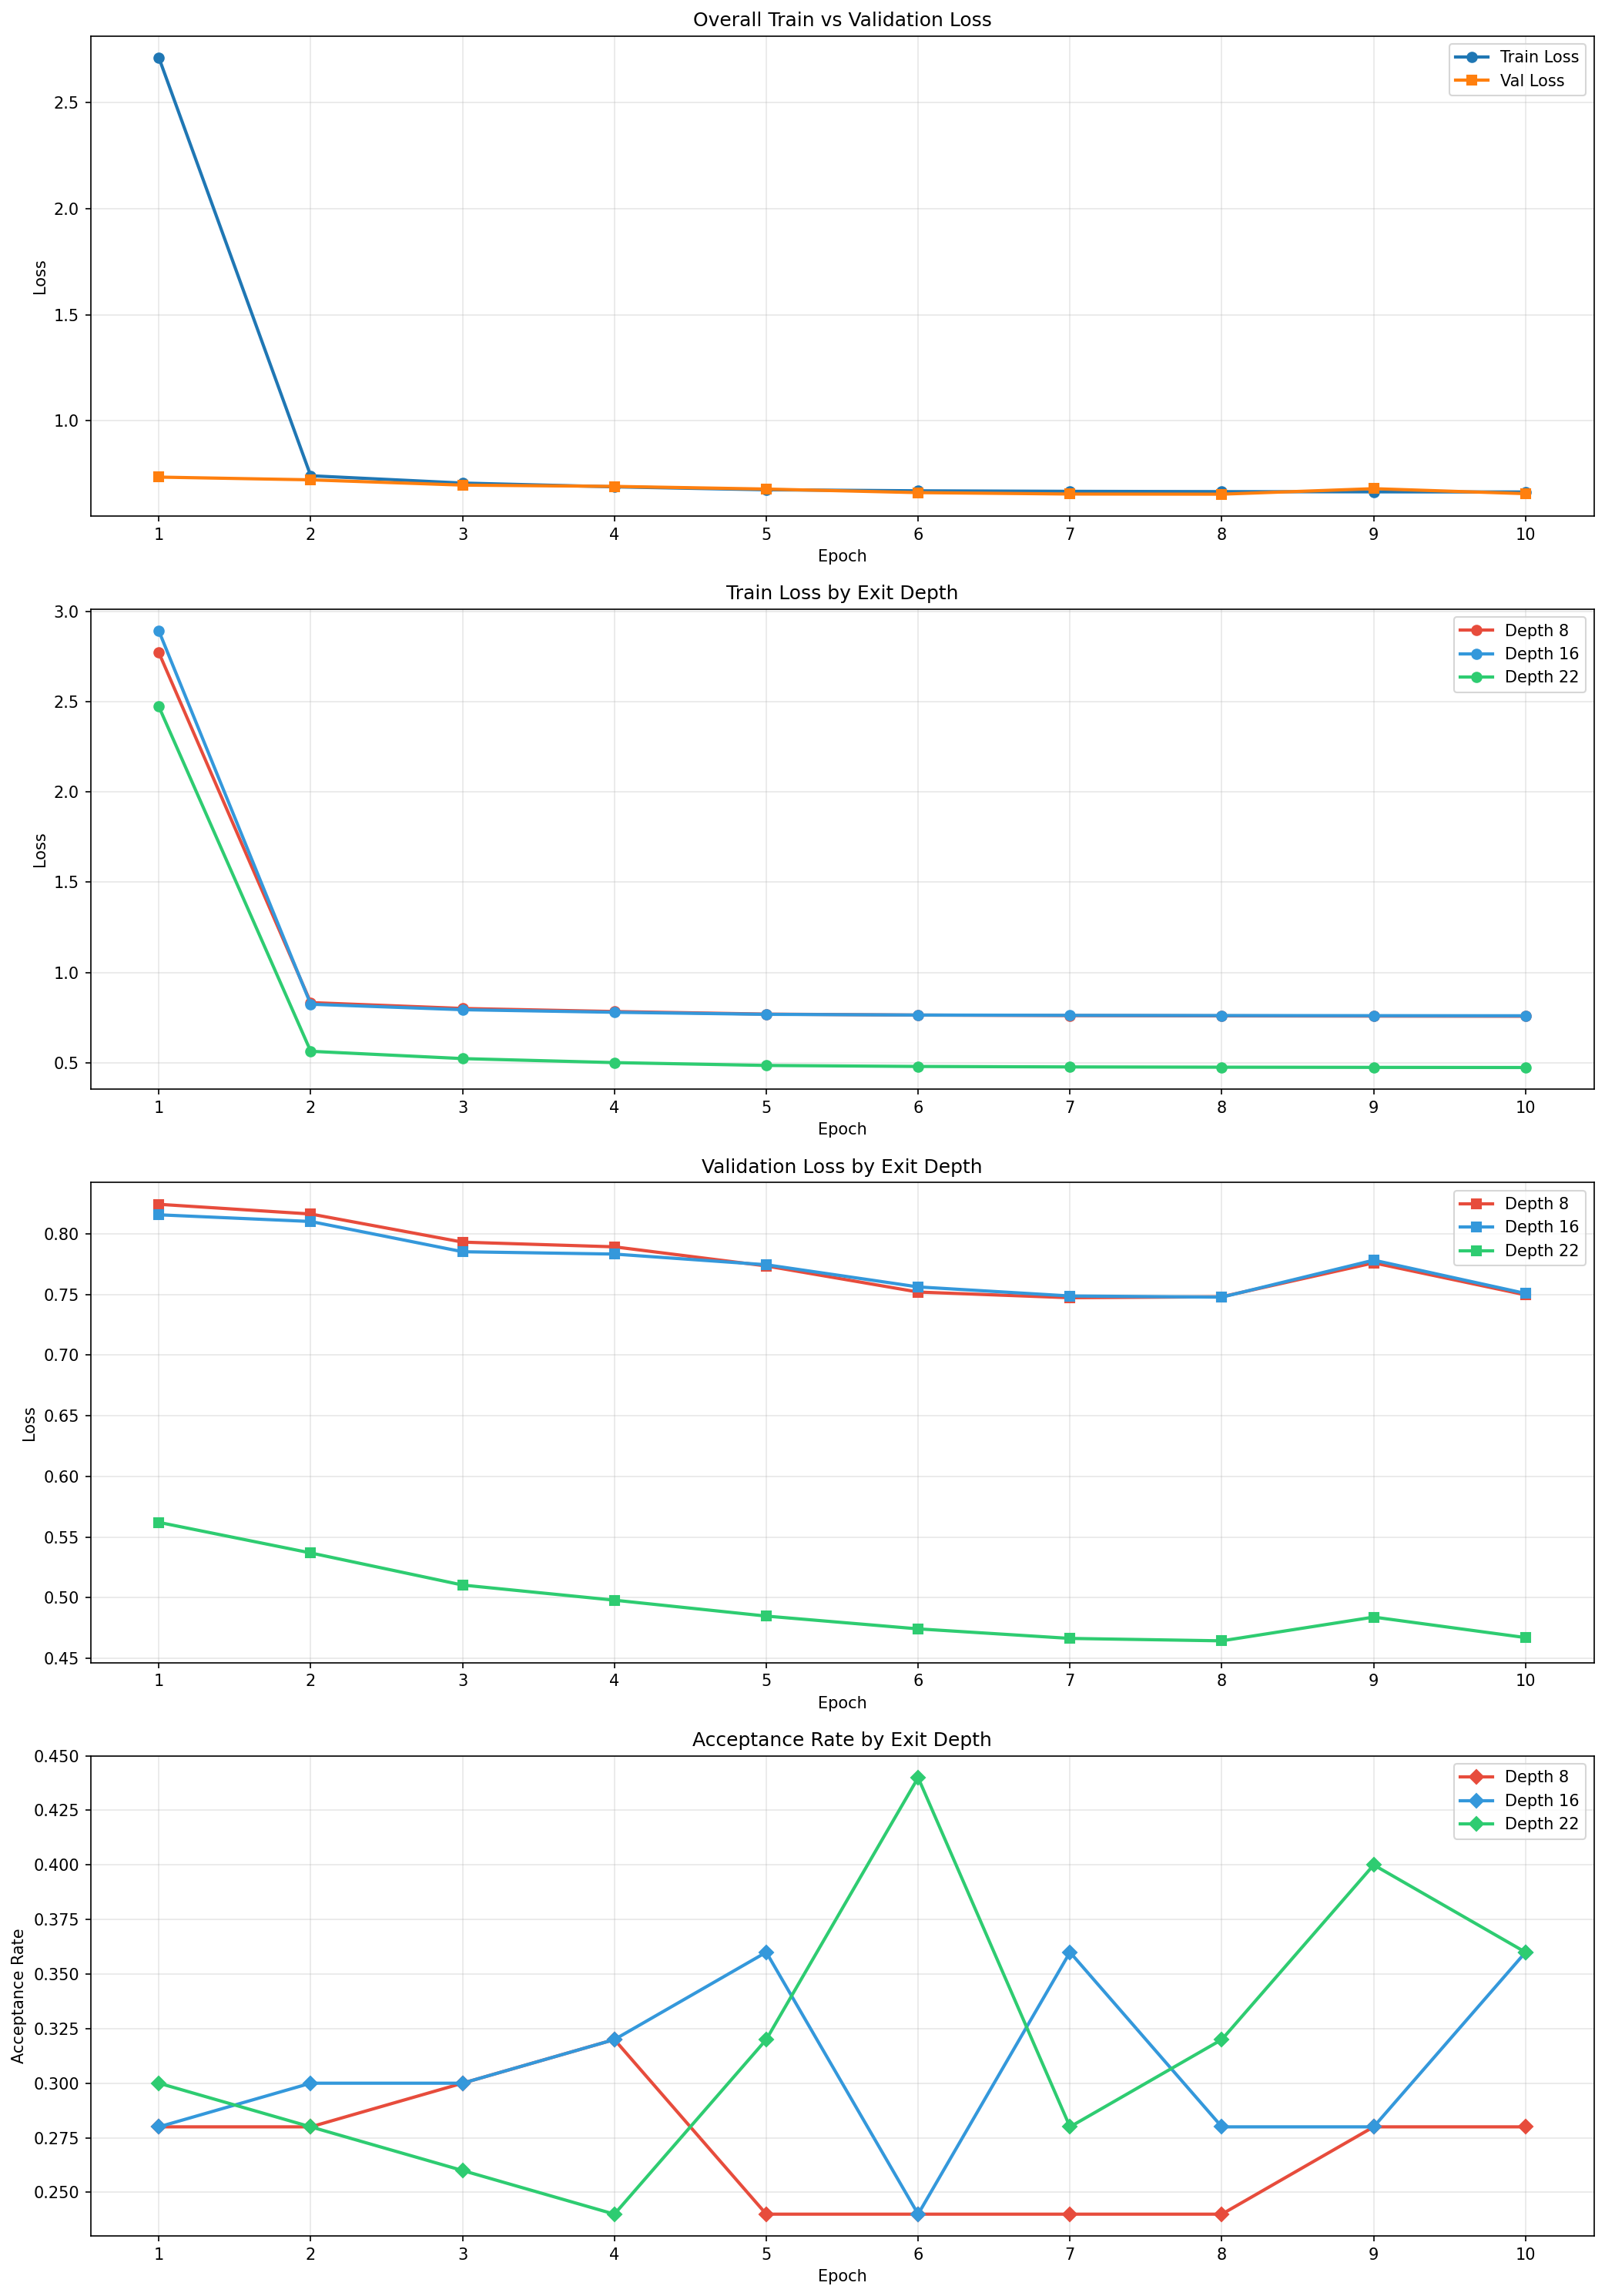
\includegraphics[width=\textwidth,height=0.88\textheight,keepaspectratio]{all_figures/loss_plots.png}
    \caption{Training dynamics over 10 epochs.  \textbf{(a)} Overall train/val KL-divergence loss showing rapid convergence (2.71 $\to$ 0.66).  \textbf{(b)} Per-depth training loss—depth 22 achieves the lowest loss ($\sim$0.47).  \textbf{(c)} Per-depth validation loss closely tracking training loss (no overfitting).  \textbf{(d)} Acceptance rate $\alpha$ on a subset of validation set prompts at epochs 1--10 with $K\!=\!3$ on 5 Hindi prompts; depth 22 reaches $\alpha = 0.36$.}
    \label{fig:loss_plots}
\end{figure*}

Key observations from training:
\begin{itemize}
    \item \textbf{Rapid initial convergence}: Loss drops from 2.71 to 0.74 between epochs 1 and 2, as exit heads quickly learn to approximate the softmax distribution.
    \item \textbf{Depth 22 dominates}: The deepest exit head consistently achieves the lowest loss (0.47 at epoch 10), demonstrating that hidden states near the output carry strong predictive signal.
    \item \textbf{Depths 8 and 16 plateau similarly}: Both shallow and mid-depth heads converge to $\sim$0.76, suggesting that the information gap between layers 8 and 16 is smaller than between 16 and 22.
    \item \textbf{No significant overfitting}: Validation loss closely tracks training loss throughout, confirming that the 167K training set provides sufficient diversity for the lightweight exit heads.
\end{itemize}

Table~\ref{tab:training_final} summarises the final (epoch 10) training metrics.

\begin{table}[t]
\centering
\small
\resizebox{\columnwidth}{!}{%
\begin{tabular}{lcccc}
\toprule
\textbf{Metric} & \textbf{Overall} & \textbf{Depth 8} & \textbf{Depth 16} & \textbf{Depth 22} \\
\midrule
Train Loss & 0.664 & 0.758 & 0.760 & 0.474 \\
Val Loss   & 0.656 & 0.750 & 0.751 & 0.467 \\
\bottomrule
\end{tabular}%
}
\caption{Final training and validation KL-divergence loss after 10 epochs.}
\label{tab:training_final}
\end{table}

The acceptance rates on the subset of validation set prompts (0.24--0.44) are lower than the full inference rates because this subset uses only 5 short prompts with $K=5$ draft tokens during training. For evaluation and inference, we use $K=3$. Full-scale inference with 101 prompts yields substantially higher rates as discussed in \S\ref{sec:inference_results}.


\subsection{Large-Scale Inference Results}
\label{sec:inference_results}

We evaluated the trained model on \textbf{101 Hindi prompts} with $K = 3$ draft tokens (note: $K=5$ was used during training) and \texttt{max\_new\_tokens} $= 100$, at each of the three exit depths.  Table~\ref{tab:inference_main} presents the main results.

\begin{table}[t]
\centering
\resizebox{\columnwidth}{!}{%
\begin{tabular}{lccc}
\toprule
\textbf{Metric} & \textbf{Depth 8} & \textbf{Depth 16} & \textbf{Depth 22} \\
\midrule
Mean $\alpha$     & 0.565 $\pm$ 0.042 & 0.589 $\pm$ 0.043 & \textbf{0.646 $\pm$ 0.049} \\
Mean Speedup      & 0.41$\times$       & 0.41$\times$       & \textbf{0.47$\times$} \\
Mean EESD Time (s)& 8.15              & 11.53              & \textbf{7.18} \\
Mean AR Time (s)  & 3.33              & 4.65               & 3.36 \\
Tokens Accepted   & 10,158            & 10,177             & 10,176 \\
Tokens Drafted    & 18,090            & 17,364             & \textbf{15,843} \\
Accept Ratio      & 56.2\%            & 58.6\%             & \textbf{64.2\%} \\
Min $\alpha$      & 0.481             & 0.500              & 0.534 \\
Max $\alpha$      & 0.667             & 0.681              & 0.756 \\
\bottomrule
\end{tabular}%
}
\caption{Inference results on 101 Hindi prompts ($K=3$ for evaluation/inference, $K=5$ for training; \texttt{max\_new\_tokens}$=100$).  Depth 22 achieves the highest acceptance rate and lowest EESD inference time.  Speedup is below 1$\times$ because drafting currently runs the full model (see \S\ref{sec:methodology}).}
\label{tab:inference_main}
\end{table}


\paragraph{Key findings:}
\begin{itemize}
    \item \textbf{Depth 22 is the clear winner}: It achieves $\alpha = 0.646$ (vs.\ 0.565 for depth 8), requires the fewest draft tokens (15,843 vs.\ 18,090), and has the lowest EESD wall time (7.18s vs.\ 8.15s).
    \item \textbf{Acceptance rate scales with depth}: $\alpha$ increases monotonically from depth 8 $\to$ 16 $\to$ 22, confirming that deeper hidden states contain progressively more information aligned with the final output distribution.
    \item \textbf{Speedup is below 1$\times$}: All depths show speedup $< 1\times$ because the current implementation runs all 28 layers during drafting.  With true early-exit (exiting at layer $d$), the expected speedup at depth 22 would be approximately $\frac{28}{22} \times \alpha \approx 0.82\times$ per draft step, with further gains from parallelised verification.
    \item \textbf{Consistent performance}: The standard deviation of $\alpha$ is small (0.04--0.05), indicating robust performance across diverse Hindi prompts.
\end{itemize}

\subsection{Depth Comparison Visualisation}

Figure~\ref{fig:inference_comparison} compares the inference evaluation plots across all three depths side by side.

\begin{figure*}[p]
    \centering
    \begin{subfigure}[b]{\textwidth}
        \centering
        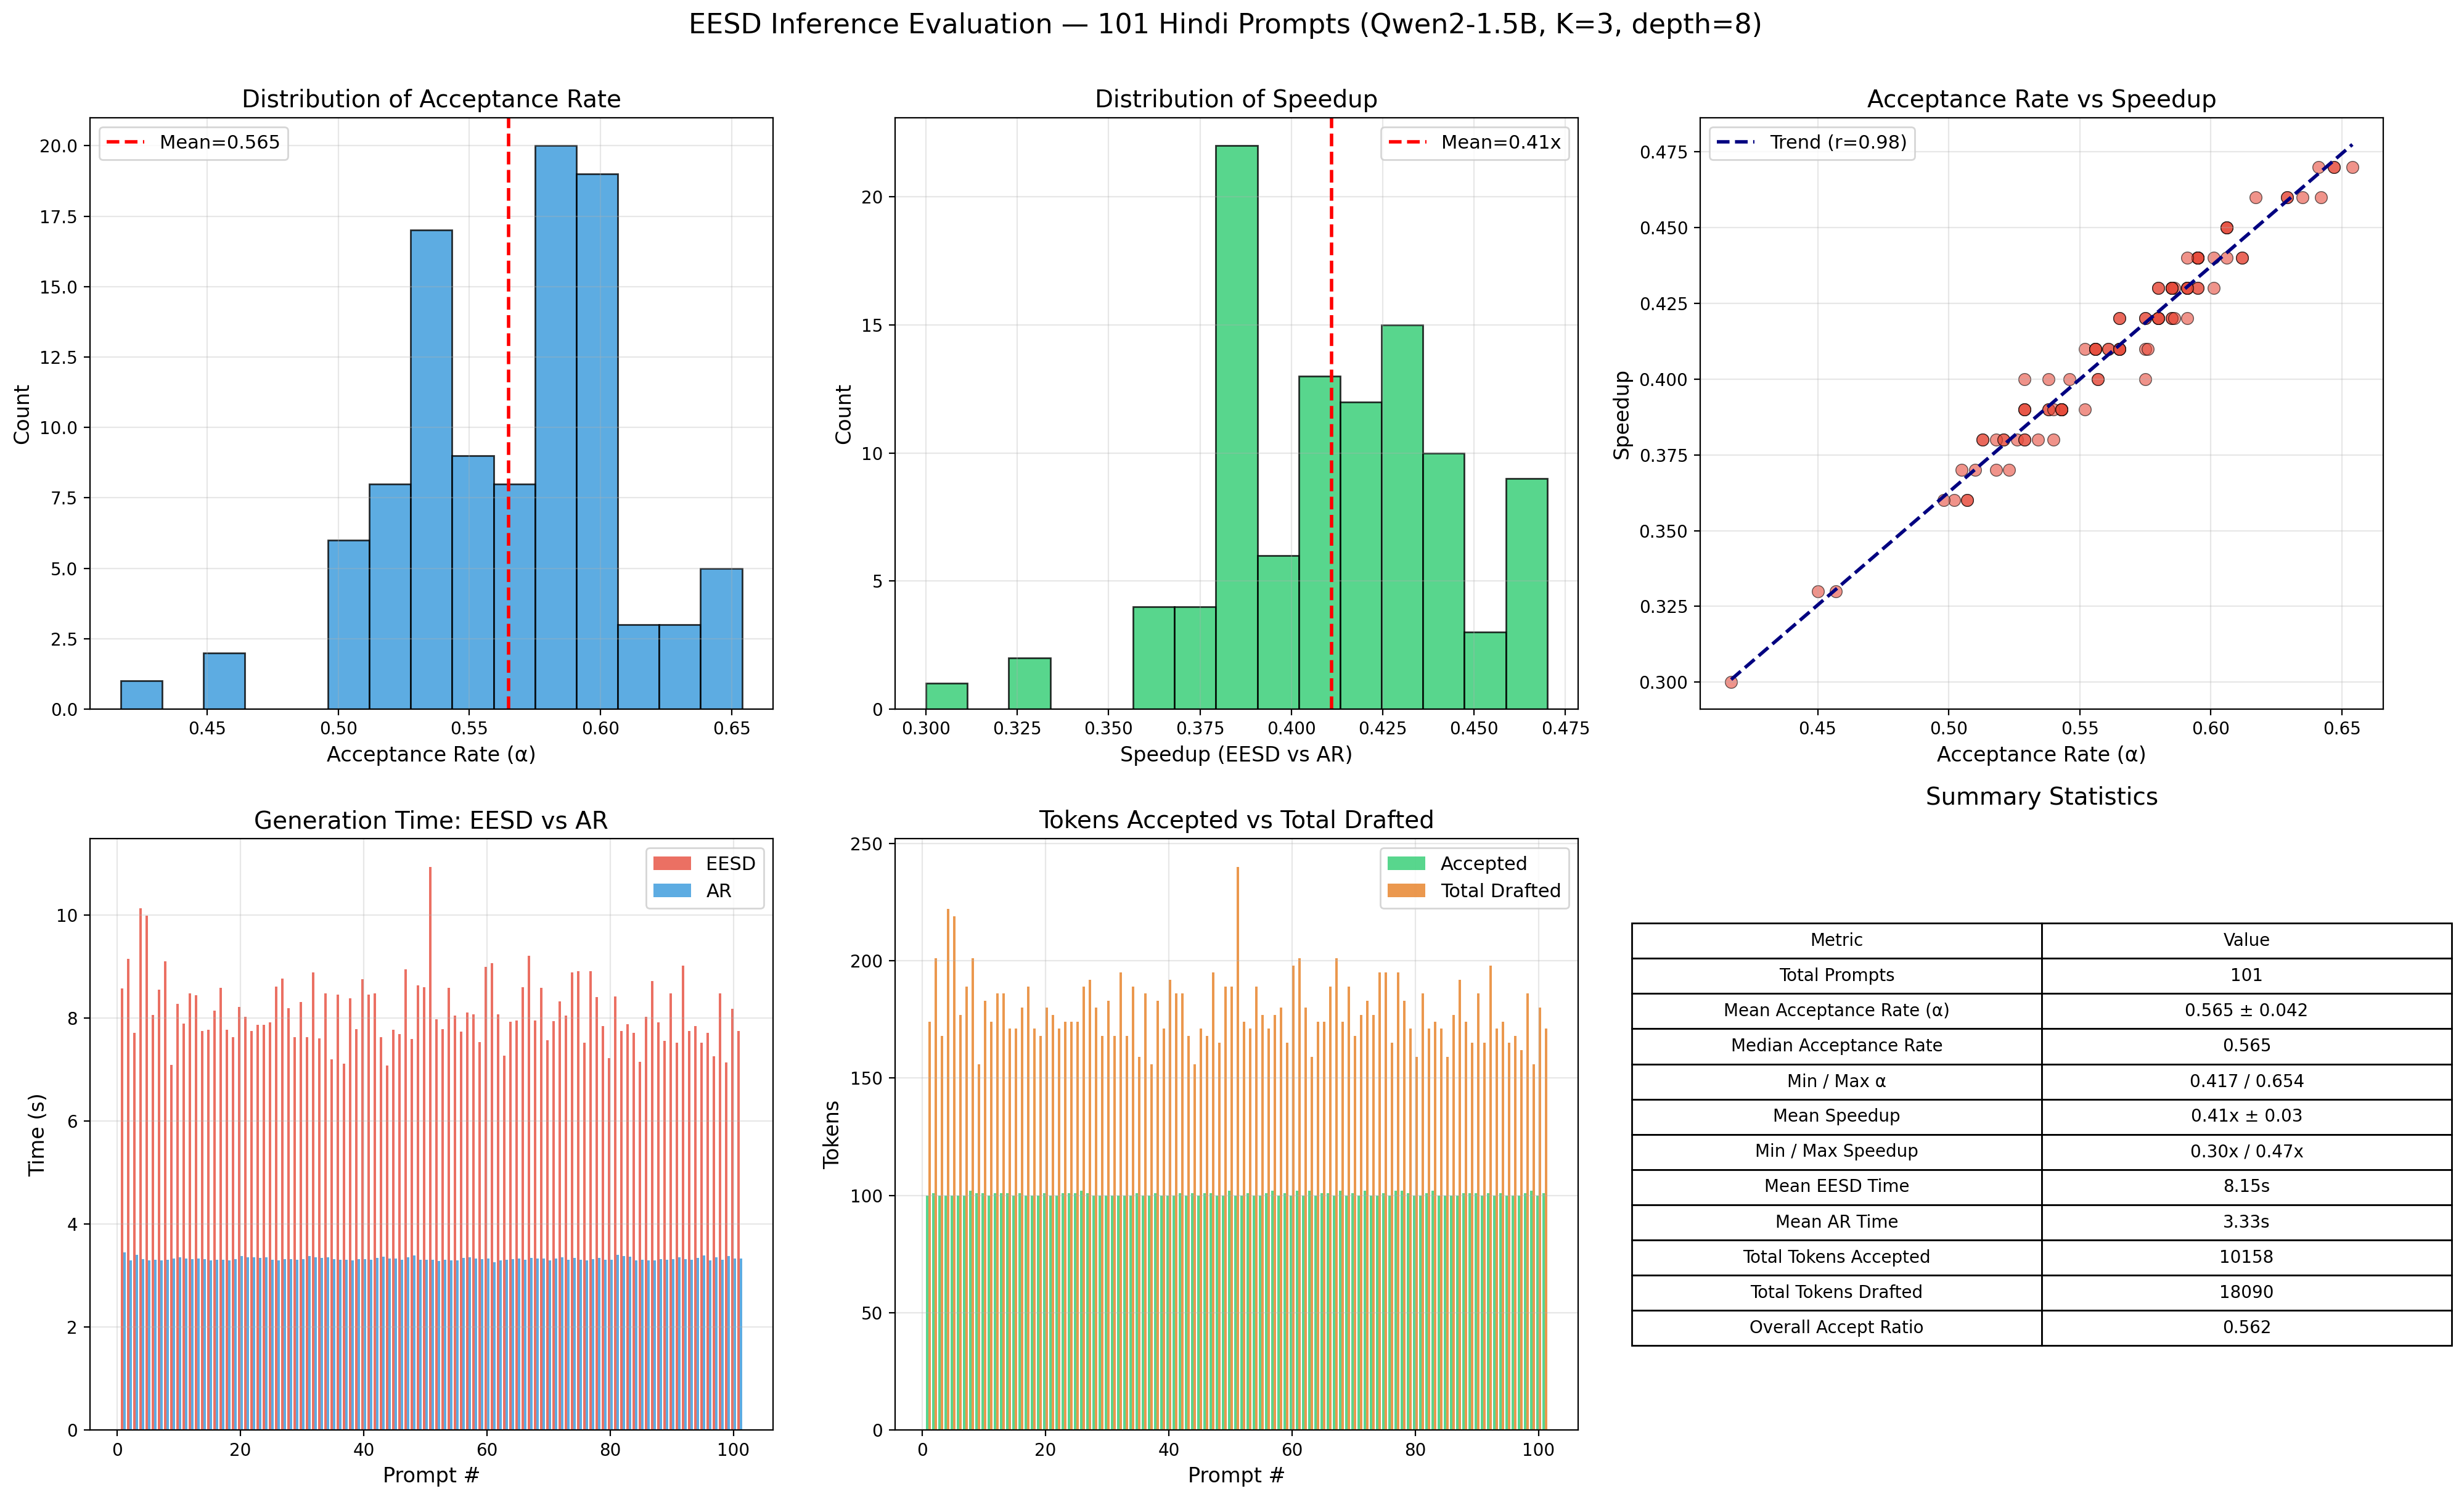
\includegraphics[width=\textwidth]{all_figures/inference_evaluation_plots_8.png}
        \caption{Depth 8}
    \end{subfigure}
    \vfill
    \begin{subfigure}[b]{\textwidth}
        \centering
        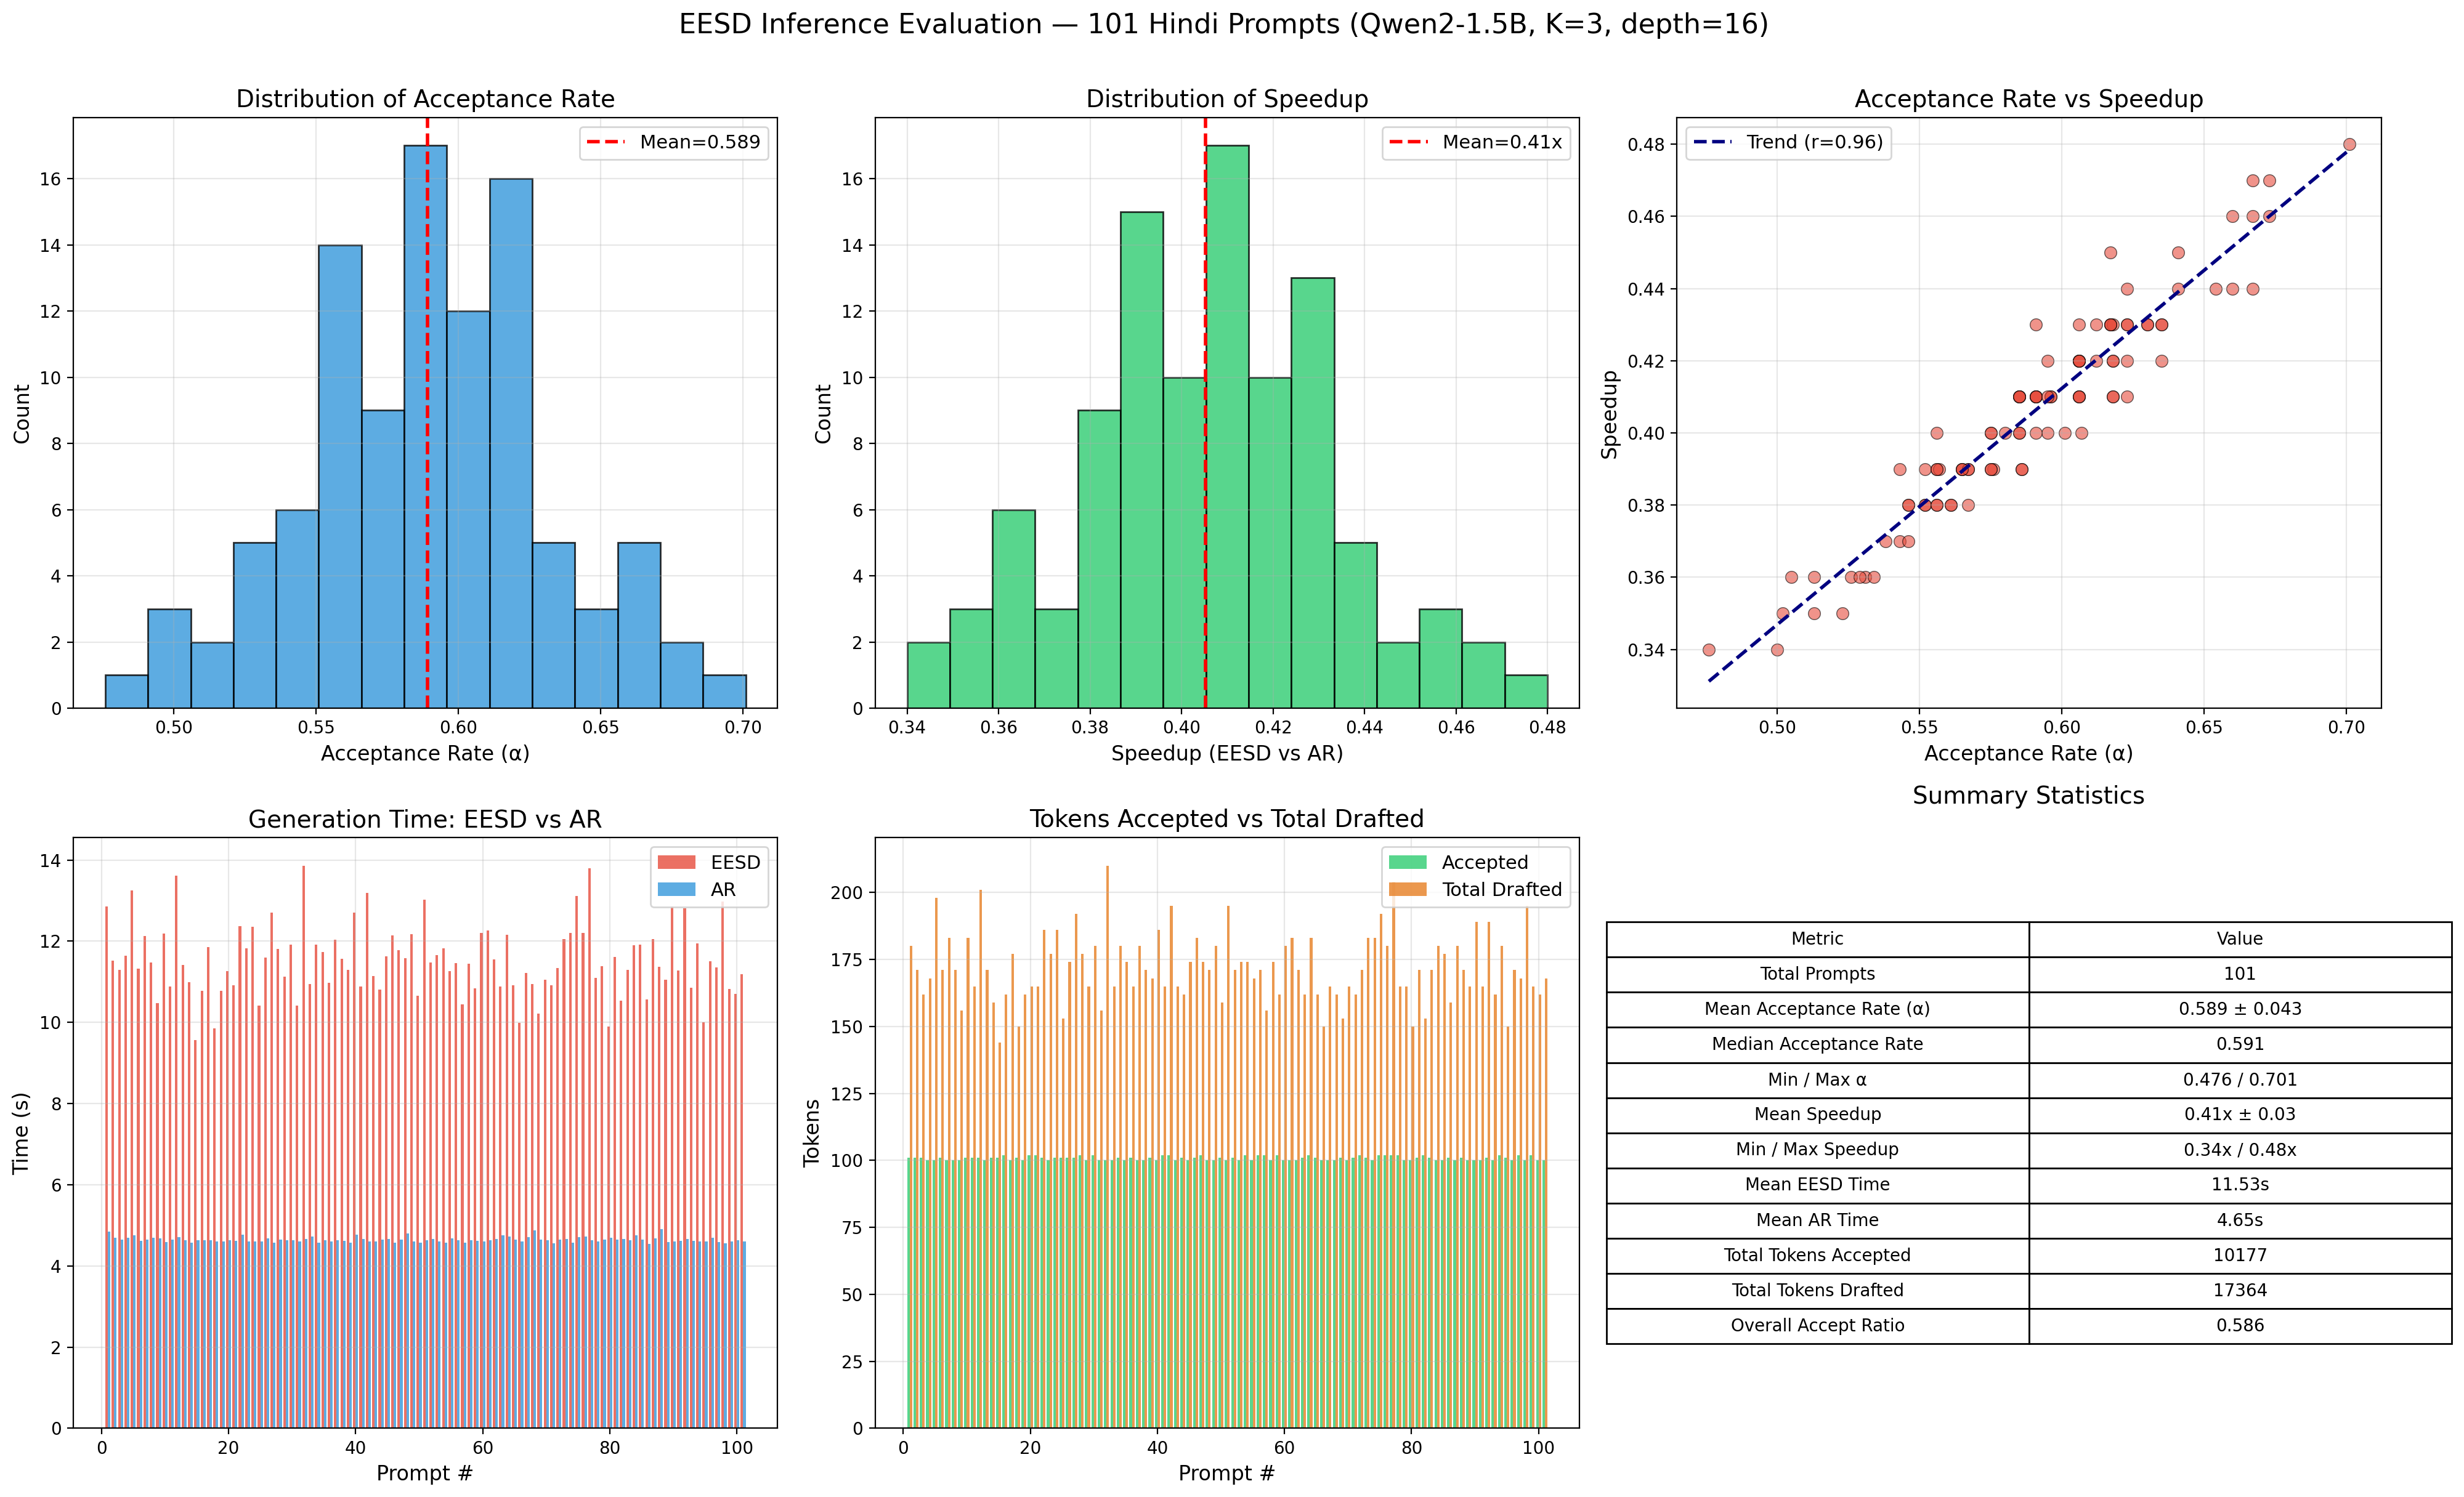
\includegraphics[width=\textwidth]{all_figures/inference_evaluation_plots_16.png}
        \caption{Depth 16}
    \end{subfigure}
    \caption{Inference evaluation plots for exit depths 8 and 16 on 101 Hindi prompts.}
    \label{fig:inference_comparison_1}
\end{figure*}

\begin{figure*}[t]
    \centering
    \begin{subfigure}[b]{\textwidth}
        \centering
        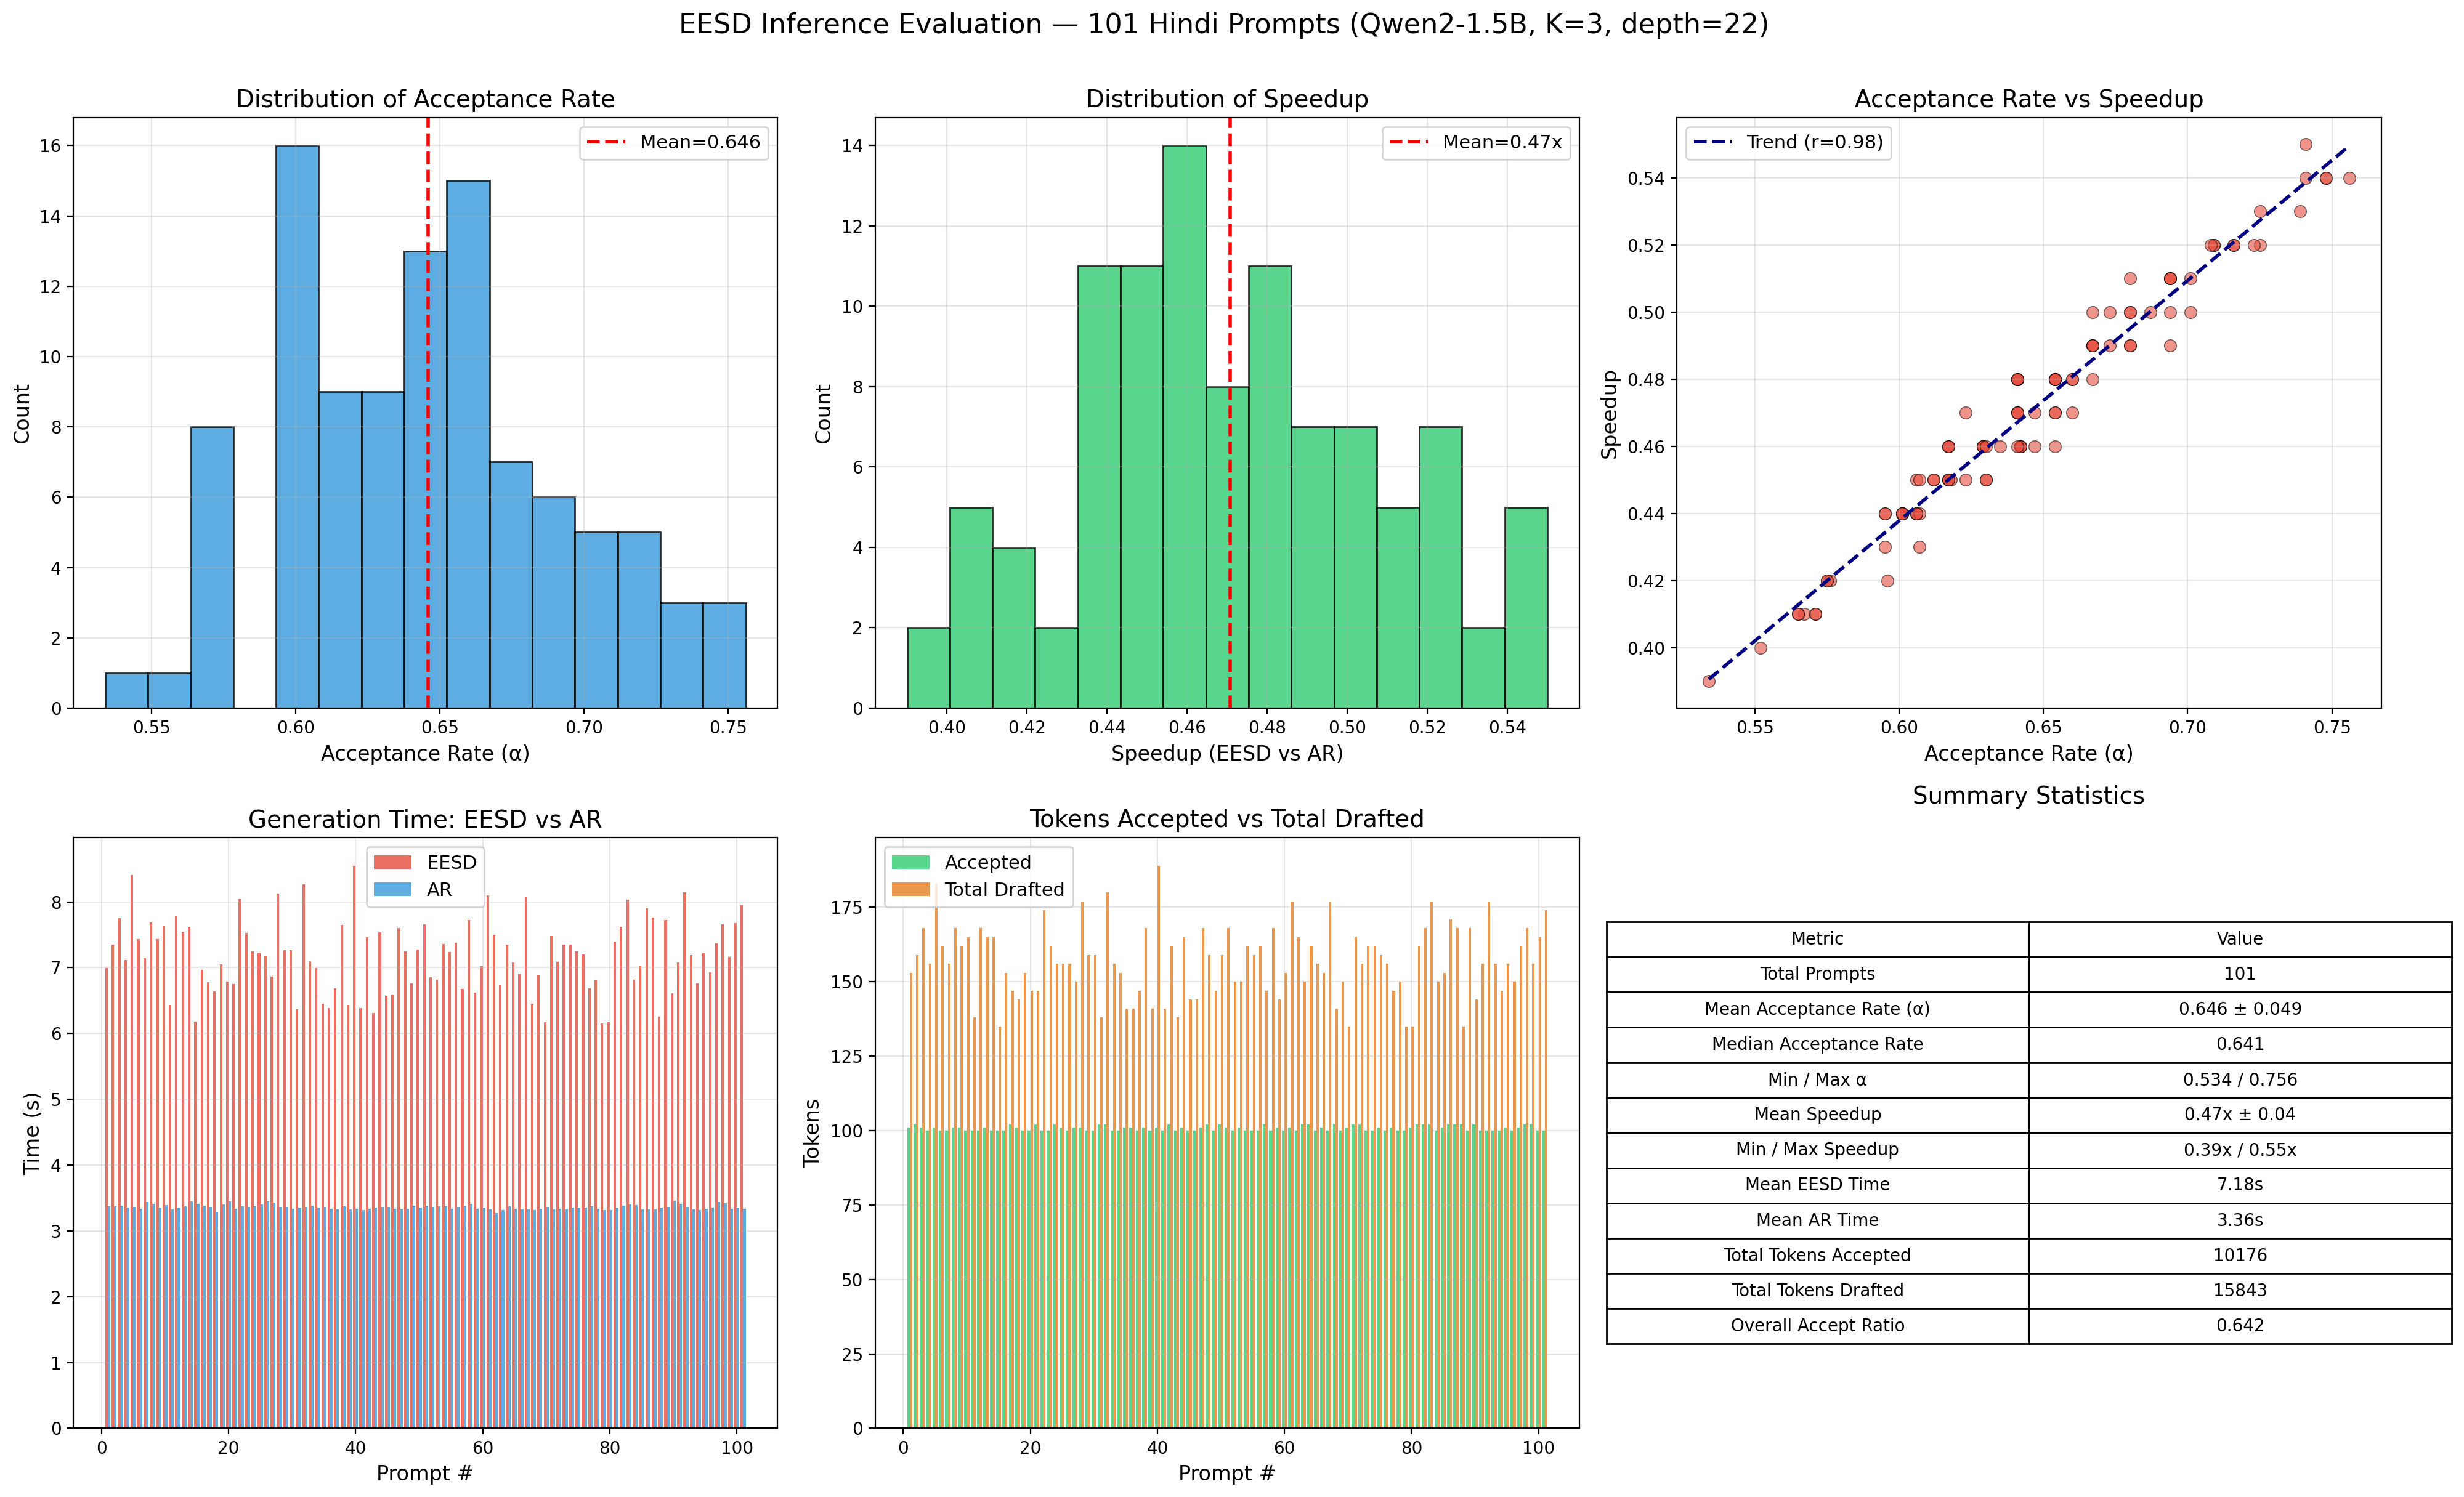
\includegraphics[width=\textwidth]{all_figures/inference_evaluation_plots_22.png}
        \caption{Depth 22}
    \end{subfigure}
    \caption{Inference evaluation plots for exit depth 22 on 101 Hindi prompts.  Depth 22 shows the tightest acceptance-rate distribution centred at a higher mean.}
    \label{fig:inference_comparison}
\end{figure*}

\subsection{Formal Evaluation (XL-Sum)}

We also ran the formal evaluation pipeline on the XL-Sum Hindi test split (Table~\ref{tab:formal_eval}), which confirms the depth ordering observed in the large-scale experiments.

\begin{table}[t]
\centering
\small
\begin{tabular}{lcccc}
\toprule
\textbf{Depth} & $\alpha$ & \textbf{Speedup} & \textbf{EESD (s)} & \textbf{AR (s)} \\
\midrule
8  & 0.531 & 0.26$\times$ & 10.38 & 2.69 \\
16 & 0.548 & 0.26$\times$ & 10.17 & 2.69 \\
22 & \textbf{0.610} & \textbf{0.29$\times$} & \textbf{9.25} & 2.69 \\
\bottomrule
\end{tabular}
\caption{Formal evaluation on XL-Sum Hindi test split.  The acceptance rate grows with depth, matching the trend in the 101-prompt experiments.}
\label{tab:formal_eval}
\end{table}


% ===================================================================
\section{Analysis and Discussion}
\label{sec:analysis}

\subsection{Why is Speedup Below (1$\times$)?}

The below-unity speedup is \emph{expected} given our implementation:

\begin{enumerate}
    \item \textbf{Draft cost equals full-model cost}: Our draft step runs all 28 layers (with a hook at the exit layer), so each draft token costs as much as an AR token.
    \item \textbf{Draft generates $K$ tokens sequentially}: For $K = 3$ draft tokens (used in evaluation/inference; $K=5$ in training), the draft phase costs $\sim 3\times$ a single AR step.
    \item \textbf{Verification adds one more full pass}: Processing the prompt + $K$ draft tokens in one forward pass costs slightly more than a single AR step due to longer sequence length.
    \item \textbf{Net cost}: $\sim (K + 1)$ forward passes to generate at most $K + 1$ tokens (if all accepted), giving theoretical speedup of $\frac{K+1}{K+1} = 1\times$ in the best case, which is never exceeded.
\end{enumerate}

With \emph{true} early exiting (running only layers 1--$d$ during drafting), the draft cost reduces to $\frac{d}{L}$ of a full pass, giving a theoretical maximum speedup of:
\begin{equation}
    S_{\max} = \frac{K \cdot \alpha + 1}{\frac{d}{L} \cdot K + 1}
\end{equation}

For $d = 22$, $L = 28$, $K = 3$, $\alpha = 0.646$:
\begin{equation}
    S_{\max} = \frac{3 \times 0.646 + 1}{\frac{22}{28} \times 3 + 1} = \frac{2.938}{3.357} \approx 0.88\times
\end{equation}

For shallower exits like $d = 8$ with the same $\alpha$:
\begin{equation}
    S_{\max} = \frac{3 \times 0.565 + 1}{\frac{8}{28} \times 3 + 1} = \frac{2.695}{1.857} \approx 1.45\times
\end{equation}

This analysis reveals the depth--speed trade-off: shallow exits enable larger speedups \emph{if} their acceptance rate is sufficient, while deep exits have higher $\alpha$ but less room for latency reduction.

\subsection{Distribution Alignment Quality}

The acceptance rate $\alpha$ measures how well the exit head's output distribution matches the full model.  Our results show:
\begin{itemize}
    \item At depth 22: $\alpha = 0.646$ (64.2\% of drafted tokens accepted).
    \item At depth 16: $\alpha = 0.589$ (58.6\%).
    \item At depth 8: $\alpha = 0.565$ (56.2\%).
\end{itemize}
The acceptance rate $\alpha$ measures how well the exit head's output distribution matches the full model.  Our results from the 101-prompt inference evaluation (Table~\ref{tab:inference_main}) \\
These rates are \emph{encouraging} for a 1.5B model with only 10 epochs of training.  For comparison, the original EESD paper reports $\alpha \approx 0.75$--$0.85$ on English with LLaMA-2-7B, suggesting that (a) larger models have more informative intermediate representations, and (b) Hindi morphology may pose additional challenges.

\subsection{Hindi-Specific Considerations}

Hindi's agglutinative morphology means that token-level predictions are harder than in English:
\begin{itemize}
    \item Inflected verb forms (e.g., \texthindi{करता}/\texthindi{करती}/\texthindi{करते}) require the model to predict agreement with subject gender and number.
    \item Postpositions (\texthindi{में}, \texthindi{को}, \texthindi{से}) interact with preceding noun forms.
    \item Compound words are common and tokenised as single or paired subword units.
\end{itemize}

Our morphological evaluation on XL-Sum (Table~\ref{tab:formal_eval}) shows $\alpha = 0.533$ on a mixed token category, indicating room for improvement in handling morphologically complex structures.


% ===================================================================
\section{Implementation Details}
\label{sec:implementation}

\subsection{Codebase Structure}

The project is organised as a Python package:

\begin{itemize}
    \item \texttt{src/model.py}: \texttt{EarlyExitLM} class with exit-head attachment, \texttt{draft()}, and \texttt{verify()} methods.
    \item \texttt{src/train.py}: Distillation training loop with gradient accumulation, mixed-precision, checkpoint saving.
    \item \texttt{src/inference.py}: \texttt{eesd\_generate()} and \texttt{autoregressive\_generate()} functions.
    \item \texttt{src/evaluate.py}: Depth analysis and morphological evaluation pipelines.
    \item \texttt{src/data.py}: Data loaders for AI4Bharat IndicCorpv2 (train) and XL-Sum Hindi (eval).
    \item \texttt{configs/default.yaml}: All hyperparameters.
\end{itemize}



\subsection{Reproducibility}

All code, configs, trained checkpoints, and evaluation logs are available in our GitHub repository .  The \texttt{configs/default.yaml} specifies all hyperparameters, and \texttt{requirements.txt} pins all dependencies.


% ===================================================================
\section{Progress and Timeline}
\label{sec:progress}

\subsection{Completed Objectives}

\begin{enumerate}
    \item[\checkmark] Literature review on speculative decoding and early exiting.
    \item[\checkmark] Full EESD implementation (model, training, inference, evaluation).
    \item[\checkmark] Data pipeline for AI4Bharat IndicCorpv2 (Hindi) and XL-Sum.
    \item[\checkmark] Exit head training for 10 epochs on 167K Hindi sentences.
    \item[\checkmark] Large-scale inference evaluation on 101 Hindi prompts at depths 8, 16, and 22.
    \item[\checkmark] Formal evaluation pipeline with depth analysis and morphological analysis.
    \item[\checkmark] Comprehensive result analysis and visualisation.
\end{enumerate}

\subsection{Ongoing Work}

\begin{enumerate}
    \item Training for additional epochs to see if acceptance rates improve further (loss was still decreasing at epoch 10).
    \item Exploring $K > 3$ draft lengths to evaluate the impact on acceptance rate and speedup.
    \item Implementing the Thompson Sampling controller from the original paper for dynamic depth selection.
\end{enumerate}

\subsection{Planned Work}

\begin{enumerate}
    \item Integrate true early-exit inference (custom forward pass that stops at layer $d$) to achieve $> 1\times$ speedup.
    \item Comparisons with an external draft model (e.g., Qwen2-0.5B) as baseline.
    \item Morphological stratification of acceptance rates (verbs vs.\ postpositions vs.\ compounds).
    
\end{enumerate}


\subsection{Timeline}


\begin{table}[h]
\centering
\small
\resizebox{\columnwidth}{!}{%
\begin{tabular}{ll}
\toprule
\textbf{Week} & \textbf{Task} \\
\midrule
1--2 & Literature review, environment setup \\
3--4 & EESD implementation (model + training) \\
5--6 & Data pipeline, initial training (3 epochs) \\
7--8 & Extended training (10 epochs), inference eval \\
9--10 & True early-exit inference, Thompson Sampling \\
11--12 & Ablation studies, cross-lingual experiments \\
13--14 & Final evaluation, report writing \\
\bottomrule
\end{tabular}%
}
\caption{Project timeline.  Weeks 1--8 are completed; weeks 9--14 are planned.}
\label{tab:timeline}
\end{table}


% ===================================================================
\section{Conclusion}
\label{sec:conclusion}

We have implemented Early-Exit Speculative Decoding (EESD) for Hindi text generation using Qwen2-1.5B, training lightweight exit heads at layers 8, 16, and 22 via KL-divergence distillation.  Our experiments on 101 Hindi prompts demonstrate that the exit heads effectively approximate the full model's output distribution, with the deepest exit (layer 22) achieving $\alpha = 0.646$ and accepting 64.2\% of drafted tokens.

While our current speedup measurements are below $1\times$ due to the full-model forward pass during drafting, the strong acceptance rates validate the core EESD approach for Hindi.  With true early-exit inference—where only the first $d$ layers are executed during drafting—we project speedups of up to $1.45\times$ for the depth-8 exit head.

This work demonstrates the viability of self-speculative decoding for morphologically rich languages and lays the groundwork for deployment-ready EESD systems that require no external draft model.


% ===================================================================
\begin{thebibliography}{23}
\expandafter\ifx\csname natexlab\endcsname\relax\def\natexlab#1{#1}\fi

\bibitem[{Bae et~al.(2023)Bae, Ko, Song, and Yun}]{bae2023fast}
Sangmin Bae, Jongwoo Ko, Hwanjun Song, and Se-Young Yun. 2023.
\newblock \href{https://arxiv.org/abs/2310.05424}{Fast and robust early-exiting framework for autoregressive language models with synchronized parallel decoding}.
\newblock In \emph{Proceedings of EMNLP}.

\bibitem[{Cai et~al.(2024)Cai, Li, Geng, Peng, Lee, Chen, and Dao}]{cai2023medusa}
Tianle Cai, Yuhong Li, Zhengyang Geng, Hongwu Peng, Jason D. Lee, Deming Chen, and Tri Dao. 2024.
\newblock \href{https://arxiv.org/abs/2401.10774}{Medusa: Simple LLM inference acceleration framework with multiple decoding heads}.
\newblock \emph{arXiv preprint arXiv:2401.10774}.

\bibitem[{Chen et~al.(2023)Chen, Borgeaud, Irving, Lespiau, Sifre, and Jumper}]{chen2023accelerating}
Charlie Chen, Sebastian Borgeaud, Geoffrey Irving, Jean-Baptiste Lespiau, Laurent Sifre, and John Jumper. 2023.
\newblock \href{https://arxiv.org/abs/2302.01318}{Accelerating large language model decoding with speculative sampling}.
\newblock \emph{arXiv preprint arXiv:2302.01318}.

\bibitem[{Doddapaneni et~al.(2023)Doddapaneni, Aralikatte, Ramesh, Goyal, Khapra, Kunchukuttan, and Kumar}]{doddapaneni2021indicnlp}
Sumanth Doddapaneni, Rahul Aralikatte, Gowtham Ramesh, Shreya Goyal, Mitesh~M. Khapra, Anoop Kunchukuttan, and Pratyush Kumar. 2023.
\newblock \href{https://huggingface.co/datasets/ai4bharat/IndicCorpV2/viewer/indiccorp_v2/hin_Deva}{Towards Leaving No Indic Language Behind: Building Monolingual Corpora, Benchmark and Models for Indic Languages}.
\newblock In \emph{Proceedings of ACL}.

\bibitem[{Elhoushi et~al.(2024)Elhoushi, Shrivastava, Liskovich, Hosmer, Wasti, Lai, Mahmoud, Acun, Agarwal, Roman, Aly, Chen, and Wu}]{elhoushi2024layerskip}
Mostafa Elhoushi, Akshat Shrivastava, Diana Liskovich, Basil Hosmer, Bram Wasti, Liangzhen Lai, Anas Mahmoud, Bilge Acun, Saurabh Agarwal, Ahmed Roman, Ahmed~A Aly, Beidi Chen, and Carole-Jean Wu. 2024.
\newblock \href{https://arxiv.org/abs/2404.16710}{LayerSkip: Enabling Early Exit Inference and Self-Speculative Decoding}.
\newblock \emph{arXiv preprint arXiv:2404.16710}.

\bibitem[{Hinton et~al.(2015)Hinton, Vinyals, and Dean}]{hinton2015distilling}
Geoffrey Hinton, Oriol Vinyals, and Jeff Dean. 2015.
\newblock \href{https://arxiv.org/abs/1503.02531}{Distilling the knowledge in a neural network}.
\newblock \emph{arXiv preprint arXiv:1503.02531}.

\bibitem[{Kim et~al.(2024)Kim, Mangalam, Moon, Malik, Mahoney, Gholami, and Keutzer}]{kim2024speculative}
Sehoon Kim, Karttikeya Mangalam, Suhong Moon, Jitendra Malik, Michael~W. Mahoney, Amir Gholami, and Kurt Keutzer. 2024.
\newblock \href{https://arxiv.org/abs/2302.07863}{Speculative decoding with big little decoder}.
\newblock In \emph{NeurIPS 2023}.

\bibitem[{Leviathan et~al.(2023)Leviathan, Kalman, and Matias}]{leviathan2023fast}
Yaniv Leviathan, Matan Kalman, and Yossi Matias. 2023.
\newblock \href{https://arxiv.org/abs/2211.17192}{Fast inference from transformers via speculative decoding}.
\newblock In \emph{Proceedings of ICML}.

\bibitem[{Liu et~al.(2024a)Liu, Wang, Wang, and Cai}]{liu2024eesd}
Jiahao Liu, Qifan Wang, Jingang Wang, and Xunliang Cai. 2024a.
\newblock \href{https://arxiv.org/abs/2406.03853}{Speculative decoding via early-exiting for faster LLM inference with Thompson Sampling control mechanism}.
\newblock In \emph{Findings of ACL 2024}.

\bibitem[{Liu et~al.(2024b)Liu, Tang, Liu, Ni, Tang, Han, and Wang}]{liu2024kangaroo}
Fangcheng Liu, Yehui Tang, Zhenhua Liu, Yunsheng Ni, Duyu Tang, Kai Han, and Yunhe Wang. 2024b.
\newblock \href{https://arxiv.org/abs/2404.18911}{Kangaroo: Lossless Self-Speculative Decoding via Double Early Exiting}.
\newblock In \emph{NeurIPS 2024}.

\bibitem[{Xu et~al.(2025)Xu, Pan, Zhou, Chen, Li, Lian, Wu, and Dai}]{xu2025specee}
Jiaming Xu, Jiayi Pan, Yongkang Zhou, Siming Chen, Jinhao Li, Yaoxiu Lian, Junyi Wu, and Guohao Dai. 2025.
\newblock \href{https://arxiv.org/abs/2504.08850}{SpecEE: Accelerating Large Language Model Inference with Speculative Early Exiting}.
\newblock In \emph{Proceedings of ISCA 2025}.

\bibitem[{Yan et~al.(2025)Yan, Agarwal, and Venkataraman}]{yan2025decoding}
Minghao Yan, Saurabh Agarwal, and Shivaram Venkataraman. 2025.
\newblock \href{https://arxiv.org/abs/2402.01528}{Decoding Speculative Decoding}.
\newblock In \emph{Proceedings of NAACL 2025}.

\bibitem[{Zhang et~al.(2023)Zhang, Wang, Li, Shou, Chen, Chen, and Mehrotra}]{zhang2023draft}
Jun Zhang, Jue Wang, Huan Li, Lidan Shou, Ke Chen, Gang Chen, and Sharad Mehrotra. 2023.
\newblock \href{https://arxiv.org/abs/2309.08168}{Draft \& verify: Lossless large language model acceleration via self-speculative decoding}.
\newblock \emph{arXiv preprint arXiv:2309.08168}.

\bibitem[{Zhao et~al.(2025)Zhao, Pan, Han, Zhang, Sun, Huang, Zhang, Zhao, Li, Wang, Liu, and Sun}]{zhao2025frspec}
Weilin Zhao, Tengyu Pan, Xu Han, Yudi Zhang, Ao Sun, Yuxiang Huang, Kaihuo Zhang, Weilun Zhao, Yuxuan Li, Jianyong Wang, Zhiyuan Liu, and Maosong Sun. 2025.
\newblock \href{https://arxiv.org/abs/2502.14856}{FR-Spec: Accelerating Large-Vocabulary Language Models via Frequency-Ranked Speculative Sampling}.
\newblock In \emph{Proceedings of ACL 2025}.

\bibitem[{Schuster et~al.(2022)Schuster, Fisch, Gupta, Dehghani, Bahri, Tran, Tay, and Metzler}]{schuster2022confident}
Tal Schuster, Adam Fisch, Jai Gupta, Mostafa Dehghani, Dara Bahri, Vinh~Q. Tran, Yi~Tay, and Donald Metzler. 2022.
\newblock \href{https://arxiv.org/abs/2207.07061}{Confident adaptive language modeling}.
\newblock In \emph{NeurIPS 2022}.

\bibitem[{Stern et~al.(2018)Stern, Shazeer, and Uszkoreit}]{stern2018blockwise}
Mitchell Stern, Noam Shazeer, and Jakob Uszkoreit. 2018.
\newblock \href{https://arxiv.org/abs/1811.03115}{Blockwise parallel decoding for deep autoregressive models}.
\newblock In \emph{NeurIPS 2018}.

\bibitem[{Teerapittayanon et~al.(2016)Teerapittayanon, McDanel, and Kung}]{teerapittayanon2016branchynet}
Surat Teerapittayanon, Bradley McDanel, and H.~T. Kung. 2016.
\newblock \href{https://arxiv.org/abs/1709.01686}{BranchyNet: Fast inference via early exiting from deep neural networks}.
\newblock In \emph{ICPR 2016}.

\bibitem[{Xia et~al.(2024)Xia, Ge, Zeng, Tang, and Wei}]{xia2024unlocking}
Heming Xia, Tao Ge, Peiyi Wang, Si-Qing Chen, Furu Wei, and Zhifang Sui. 2024.
\newblock \href{https://arxiv.org/abs/2401.07851}{Unlocking efficiency in large language model inference: A comprehensive survey of speculative decoding}.
\newblock In \emph{Findings of ACL 2024}.

\bibitem[{Xin et~al.(2020)Xin, Tang, Lee, Yu, and Lin}]{xin2020deebert}
Ji~Xin, Raphael Tang, Jaejun Lee, Yaoliang Yu, and Jimmy Lin. 2020.
\newblock \href{https://arxiv.org/abs/2004.12993}{DeeBERT: Dynamic early exiting for accelerating BERT inference}.
\newblock In \emph{Proceedings of ACL}.

\bibitem[{Yang et~al.(2024)Yang, Yang, Hui, Zheng, Yu, Zhou, Liu, Huang, Yu, Li, Zhu, Zhang, Press, Li, and Lin}]{yang2024qwen2}
An~Yang, Baosong Yang, Binyuan Hui, Bo~Zheng, Bowen Yu, Chang Zhou, Chengpeng Li, Chengyuan Li, Dayiheng Liu, Fei Huang, Guanting Dong, Haoran Wei, Huan Lin, Jialong Tang, Jialin Wang, et~al. 2024.
\newblock \href{https://arxiv.org/abs/2407.10671}{Qwen2 technical report}.
\newblock \emph{arXiv preprint arXiv:2407.10671}.

\bibitem[{Zhou et~al.(2024)Zhou, Liu, Ning, Yang, Du, Han, Wei, Fan, Ai, Chen, et~al.}]{zhou2024survey}
Ce~Zhou, Qian Liu, Peng Ning, Yingyao Yang, Chenshu Du, Yuhua Han, Shuyuan Wei, Jia Fan, Shanghang Ai, Yaowei Chen, et~al. 2024.
\newblock \href{https://arxiv.org/abs/2303.18223}{A survey of large language models}.
\newblock \emph{arXiv preprint arXiv:2303.18223}.

\bibitem[{Hasan et~al.(2021)Hasan, Bhattacharjee, Islam, Mubasshir, Li, Kang, Rahman, Shahriyar, Solorio, and Rig}]{hasan2021xlsum}
Tahmid Hasan, Abhik Bhattacharjee, Md.~Saiful Islam, Kazi Mubasshir, Yuan-Fang Li, Yong-Bin Kang, M.~Sohel Rahman, Rifat Shahriyar, Thamar Solorio, and Stephan Rig. 2021.
\newblock \href{https://arxiv.org/abs/2106.13822}{XL-Sum: Large-scale multilingual abstractive summarization for 44 languages}.
\newblock In \emph{Findings of ACL 2021}.

\bibitem[{Loshchilov and Hutter(2019)}]{loshchilov2019adamw}
Ilya Loshchilov and Frank Hutter. 2019.
\newblock \href{https://arxiv.org/abs/1711.05101}{Decoupled weight decay regularization}.
\newblock In \emph{ICLR 2019}.

\end{thebibliography}
\end{document}
